% =====================================================================
% THIS FILE IS THE SOURCE. Edit it, then rebuild the PDF with:
%     bash tools/compile.sh Unit_05_When_a_Line_Is_Not_Enough
%
% Figures are the fig_u5_*.pdf files in this folder, from
% tools/make_unit05_slide_figs.py. The data is made up, and comes from
% tools/make_lawn_data.py.
% =====================================================================
\documentclass[aspectratio=169]{beamer}
\usetheme{default}
\usefonttheme{professionalfonts}
\usepackage{amsmath, amssymb, amsfonts}
\usepackage{graphicx}
\usepackage{booktabs}
\renewcommand{\arraystretch}{1.2}
\usepackage{array}
\newcolumntype{L}[1]{>{\raggedright\arraybackslash}p{#1}}
\usepackage{bm}
\usepackage{hyperref}

\mode<presentation> {
    \usetheme{Frankfurt}
    \usecolortheme{default}
}

\newcommand{\xbar}{\bar{x}}
\newcommand{\SE}{\mathrm{SE}}
\newcommand{\se}{\widehat{\SE}}

\newenvironment{principle}[1]{\begin{block}{\textbf{Principle:} #1}}{\end{block}}
\newenvironment{trap}[1]{\begin{alertblock}{\textbf{Trap:} #1}}{\end{alertblock}}
\newenvironment{practice}[1]{\begin{exampleblock}{\textbf{In practice:} #1}}{\end{exampleblock}}
\newenvironment{interview}[1]{\begin{exampleblock}{\textbf{You may be asked:} #1}}{\end{exampleblock}}
\newenvironment{yourturn}[1]{%
  \setbeamercolor{block title}{fg=white,bg=orange!80!black}%
  \setbeamercolor{block body}{bg=orange!12}%
  \begin{block}{\textbf{Your turn:} #1}}{\end{block}}
\newenvironment{llmcheck}[1]{%
  \setbeamercolor{block title}{fg=white,bg=violet!75!black}%
  \setbeamercolor{block body}{bg=violet!10}%
  \begin{block}{\textbf{LLM check:} #1}}{\end{block}}

\title{When a Line Is Not Enough}
\subtitle{Unit 5: Fixing a Model, and Letting a Tree Show You Where to Look}
\author{Stat 220 \textbar{} Statistics for Data Science}
\date{}

\begin{document}

\begin{frame}
  \titlepage
\end{frame}

% ======================================================================
\section{Why}
% ======================================================================
\begin{frame}{Where we left off}
\begin{itemize}
  \item Units 3 and 4 fitted straight lines, read the coefficients, and chose which predictors
        to keep.
  \item All of that assumed the straight line was roughly the right shape, and that the spread
        around it was roughly constant.
  \item This unit is what you do when it is not: how to tell, what to change, and what to reach
        for when a line will not do the job at all.
\end{itemize}
\end{frame}

\begin{frame}{What this unit gives you}
\begin{columns}[T]
\begin{column}{0.5\textwidth}
\textbf{Things to know}
\begin{itemize}\small
  \item what each broken assumption looks like in a residual plot
  \item when a log fixes spread that grows, and how to read the result
  \item how to put curves and interactions into a linear model
  \item how a decision tree is built, one split at a time
  \item what a tree is good at, and where it falls down
  \item how to use a tree to find terms worth adding to a regression
\end{itemize}
\end{column}
\begin{column}{0.5\textwidth}
\textbf{Mistakes to stop making}
\begin{itemize}\small
  \item reading coefficients off a model whose residuals are patterned
  \item taking logs and then reporting the coefficient in the original units
  \item adding squared terms everywhere instead of looking first
  \item reading a tree's splits as effects
  \item expecting a tree to predict outside the range of the data
  \item choosing between a tree and a regression on their fit to the same rows
\end{itemize}
\end{column}
\end{columns}
\end{frame}

\begin{frame}{The data for this unit}
\texttt{lawn\_jobs.csv}: 700 completed jobs at a lawn care company.
\begin{center}\small
\begin{tabular}{L{0.26\textwidth} L{0.62\textwidth}}
\toprule
\textbf{Column} & \textbf{What it is} \\
\midrule
\texttt{minutes} & time on the property, the outcome \\
\texttt{lot\_sqft} & size of the lot \\
\texttt{slope} & flat, moderate, or steep \\
\texttt{obstacles} & trees, beds and play sets to mow around \\
\texttt{gated} & 1 if the property is behind a gate \\
\texttt{crew\_size} & people on the job, 1 to 3 \\
\texttt{invoice\_id}, \texttt{customer\_rating} & also recorded \\
\bottomrule
\end{tabular}
\end{center}
\vspace{0.3em}
The company schedules by estimated time, so a prediction that is off by a third ruins the
afternoon.
\end{frame}

% ======================================================================
\section{When the line is wrong}
% ======================================================================
\begin{frame}{What the residuals are telling you}
A residual plot is the model showing you what it could not explain. Four things turn up.
\begin{center}\small
\begin{tabular}{L{0.26\textwidth} L{0.62\textwidth}}
\toprule
\textbf{What you see} & \textbf{What it means} \\
\midrule
a shapeless cloud & the shape you fitted is about right \\
a curve or a U & the relationship bends and the line does not \\
a fan or a wedge & the spread grows with the size of the prediction \\
one point far away & a single case is pulling the fit toward itself \\
\bottomrule
\end{tabular}
\end{center}
\vspace{0.2em}
\begin{principle}{look before you read}
The coefficient table does not know whether the shape is right. The residual plot is the only
place that shows you.
\end{principle}
\end{frame}

\begin{frame}{The four pictures}
\centering
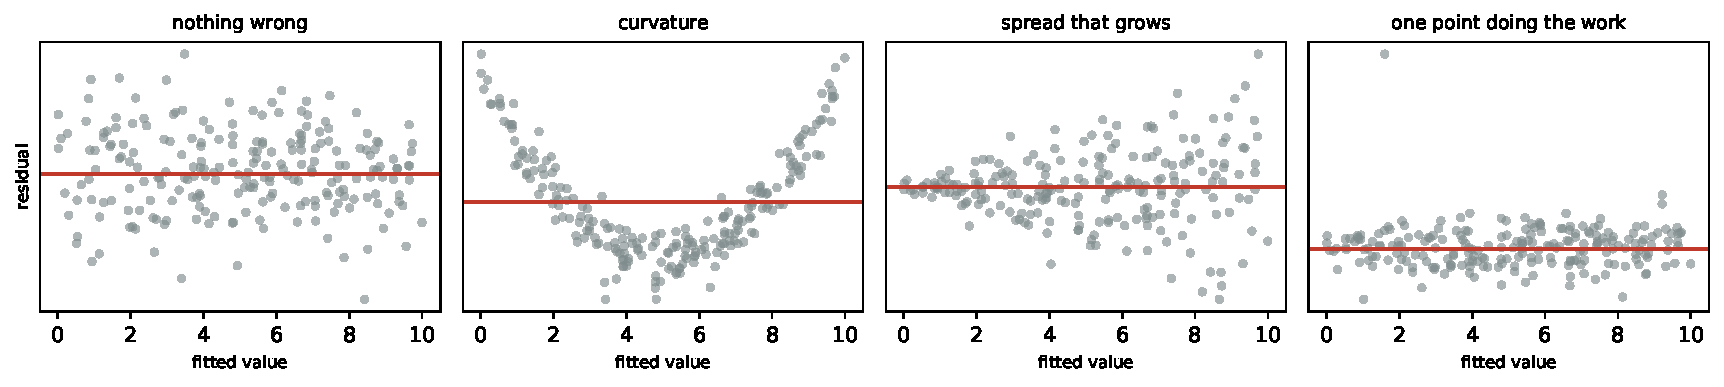
\includegraphics[width=\textwidth]{fig_u5_diagnostics.pdf}
\vspace{0.4em}
\begin{minipage}{0.92\textwidth}\small
Only the first one is a model you can read coefficients from as they stand. The other three each
have a standard response, and the rest of this unit is those responses.
\end{minipage}
\end{frame}

\begin{frame}{What to do about each one}
\begin{center}\small
\begin{tabular}{L{0.24\textwidth} L{0.64\textwidth}}
\toprule
\textbf{Problem} & \textbf{Usual response} \\
\midrule
the relationship bends & add a squared term, or transform the predictor \\
spread grows with the fit & model $\log(y)$ instead of $y$ \\
one case dominates & find out what it is; report the fit with and without it \\
cases are not independent & a different family of models, named on the next slide \\
the outcome is not a number & also a different family, also next slide \\
\bottomrule
\end{tabular}
\end{center}
\vspace{0.2em}
\begin{trap}{the quiet failure}
Nothing in the output tells you any of this happened. A model with patterned residuals still
prints coefficients, p-values and an $R^2$ to three decimals.
\end{trap}
\end{frame}

\begin{frame}{Three things this course points at but does not teach}
\begin{itemize}
  \item \textbf{Time series.} Measurements on the same thing over time are not independent:
        today looks like yesterday. Unit 1 showed what that does to a p-value. Fixing it properly
        needs models built for it.
  \item \textbf{Spatial statistics.} The same problem in two dimensions: nearby places resemble
        each other. Mowing times on one street are not independent draws.
  \item \textbf{Generalized linear models.} When the outcome is a yes/no or a count, the model
        gets a different link and a different spread. Logistic regression, which Unit 10 covers,
        is one of these.
\end{itemize}
\begin{practice}{what to do when you meet one}
Recognize it, say so, and go find the right tool or the right person. Knowing that your data is
a time series is most of the battle; the rest is a course of its own.
\end{practice}
\end{frame}

% ======================================================================
\section{Transformations}
% ======================================================================
\begin{frame}{Why spread so often grows with the prediction}
\begin{itemize}
  \item A big lawn does not take a fixed number of extra minutes. It takes a percentage longer,
        and the things that go wrong on it cost a percentage too.
  \item When effects multiply rather than add, the spread around a big prediction is bigger than
        the spread around a small one. That is the fan.
  \item Taking logs turns multiplication into addition, which is exactly the shape a linear model
        is built for.
\end{itemize}
\[
   y = a \cdot b^{x} \cdot \varepsilon
   \qquad\Longrightarrow\qquad
   \log y = \log a + x\log b + \log\varepsilon
\]
\end{frame}

\begin{frame}{The same jobs, before and after}
\centering
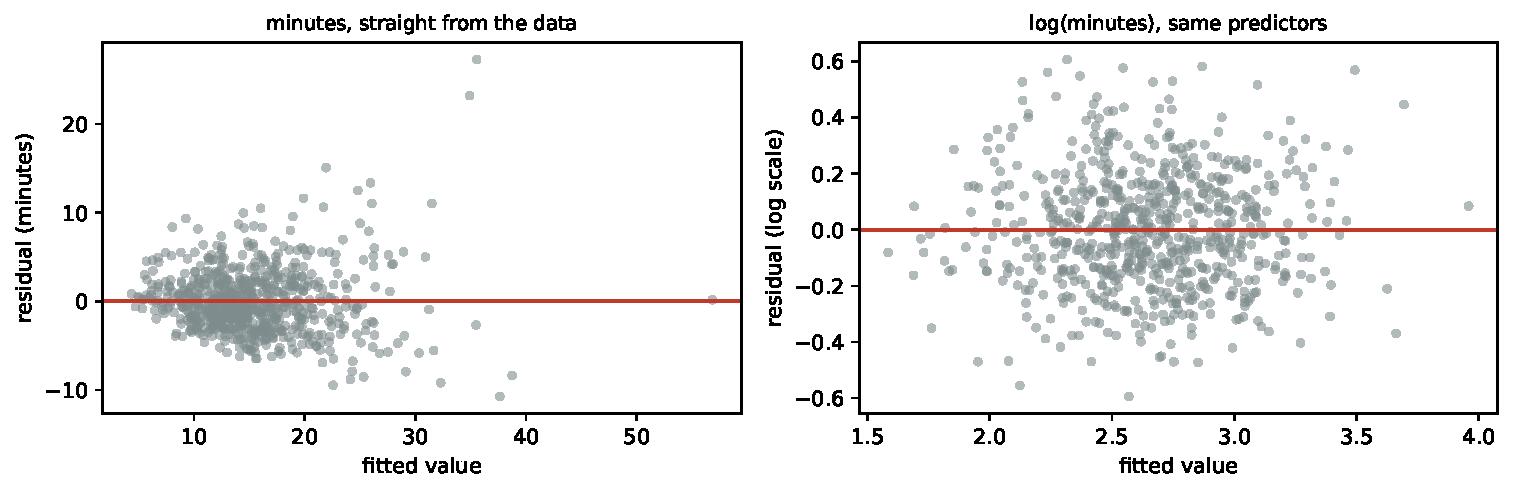
\includegraphics[width=0.94\textwidth]{fig_u5_fan.pdf}
\vspace{0.3em}
\begin{minipage}{0.94\textwidth}\small
Left: minutes on the raw scale. The spread at a 40-minute prediction is nearly twice the spread
at a 10-minute one. Right: the same predictors against $\log(\text{minutes})$. The fan is gone
and $R^2$ rises from 0.69 to 0.74.
\end{minipage}
\end{frame}

\begin{frame}{Reading a coefficient after a log}
\begin{itemize}
  \item On a logged outcome, a coefficient $b$ is a \emph{percentage}: roughly
        $100(e^{b}-1)\%$ for each one-unit change in the predictor.
  \item Gated properties have a coefficient of $0.26$, which is about \textbf{30\% longer}, not
        0.26 minutes longer.
  \item If you log the predictor too, the coefficient is a percentage for a percentage. Here the
        coefficient on $\log(\text{lot size})$ is $0.52$: a lot 10\% bigger takes about 5\%
        longer.
\end{itemize}
\begin{trap}{reporting in the wrong units}
``Gating adds 0.26'' is not a sentence about minutes, and a manager will read it as one. Convert
before you report.
\end{trap}
\end{frame}

\begin{frame}{Two things to know before you take a log}
\begin{itemize}
  \item \textbf{Zeros and negatives have no log.} Counts that include zero need a different
        answer, not $\log(y+1)$ chosen because it ran without an error.
  \item \textbf{Exponentiating a fitted value gives you back a median, not a mean.} For most
        operational questions that is fine, and it is worth knowing which one you handed over.
  \item The model is now about $\log(\text{minutes})$. Every interval and every prediction comes
        back on that scale until you convert it.
\end{itemize}
\end{frame}

\begin{frame}{Your turn \#1}
\begin{yourturn}{which fix fits which picture?}
Match each residual plot to its response:
\vspace{0.3em}
\begin{enumerate}\small
  \item The residuals fan out as the fitted value grows.
  \item The residuals form a clear arc, negative at both ends.
  \item One residual sits five times further from zero than any other.
\end{enumerate}
\vspace{0.2em}
Decide with a neighbour, and say what you would check before doing anything to number 3.
\end{yourturn}
\end{frame}

\begin{frame}{Your turn \#1: answer}
\begin{itemize}
  \item \textbf{(1) Fan.} Model the log of the outcome, then report in percentages.
  \item \textbf{(2) Arc.} The shape is wrong, not the spread. Add a squared term or transform the
        predictor.
  \item \textbf{(3) One point.} Find out what it is first. A data entry error gets fixed, a real
        unusual job gets reported both ways, and neither gets deleted because it was inconvenient.
\end{itemize}
\end{frame}

% ======================================================================
\section{Curves by hand}
% ======================================================================
\begin{frame}{Bending a line on purpose}
\centering
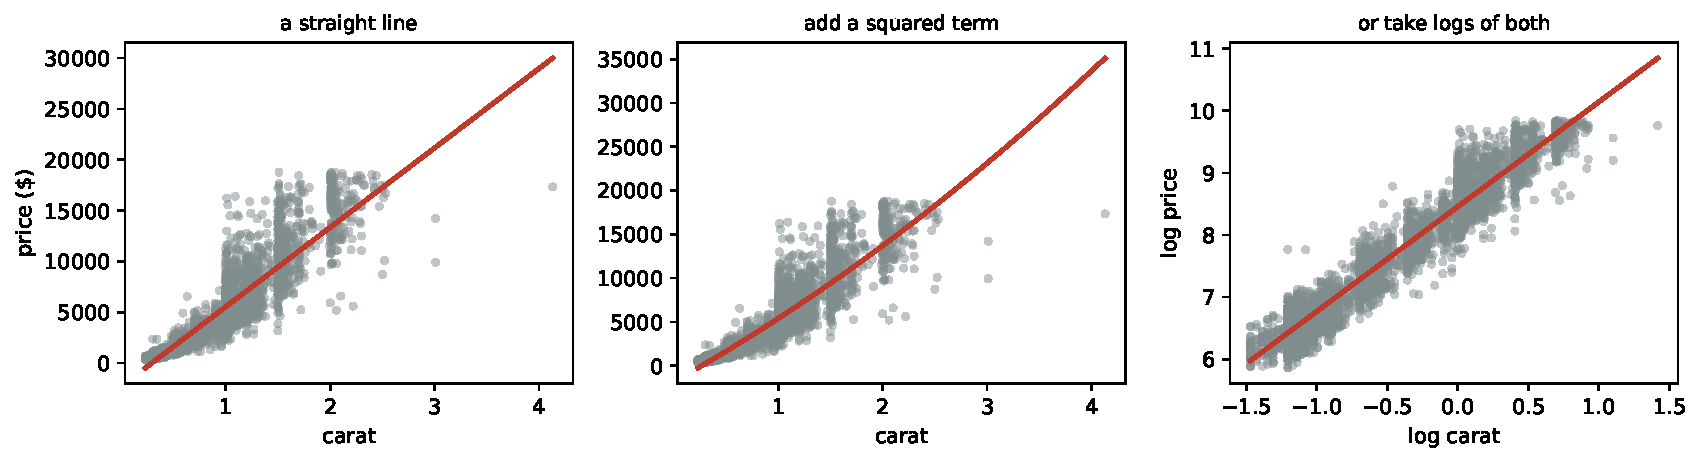
\includegraphics[width=\textwidth]{fig_u5_poly.pdf}
\vspace{0.3em}
\begin{minipage}{0.94\textwidth}\small
The same 700 jobs three ways. A straight line misses the shape at both ends. A squared term
follows it. Taking logs of both sides straightens the relationship instead of bending the model,
which is usually the better move when the cause of the curve is multiplicative.
\end{minipage}
\end{frame}

\begin{frame}{The two tools you already have}
\begin{itemize}
  \item \textbf{Polynomial terms.} Add $x^2$, and the fitted curve can bend once. Add $x^3$ and
        it can bend twice. Each is an ordinary column, and the model is still linear regression.
  \item \textbf{Interactions.} Add $x_1x_2$, and the effect of one predictor is allowed to depend
        on the other. Steep lots may cost more time only when they are also large.
  \item Both are choices \emph{you} make about shape, before fitting.
\end{itemize}
\begin{principle}{the catch}
A squared term only helps if you suspected a curve in that variable. An interaction only helps if
you suspected those two variables interact. With a dozen predictors there are far more
possibilities than you can check by hand.
\end{principle}
\end{frame}

% ======================================================================
\section{Decision trees}
% ======================================================================
\begin{frame}{A different idea entirely}
\begin{itemize}
  \item Stop writing an equation. Instead, ask a sequence of yes/no questions and read the answer
        off the end.
  \item \emph{Is the lot bigger than 11,000 square feet? If yes, is it behind a gate? If yes,
        predict 38 minutes.}
  \item That is a \textbf{decision tree}. The questions are chosen by the data, not by you, which
        is the point.
\end{itemize}
\end{frame}

\begin{frame}{One split}
\centering
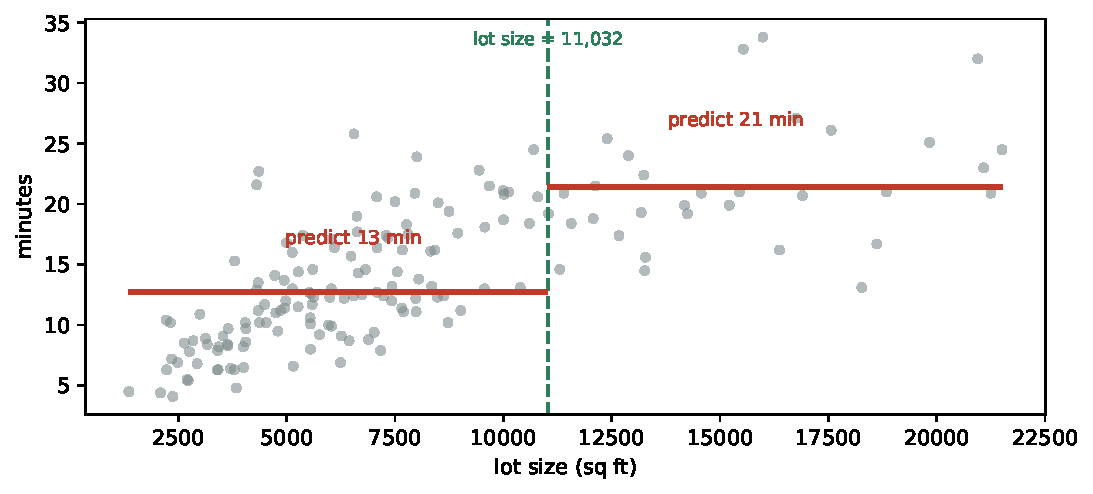
\includegraphics[width=0.82\textwidth]{fig_u5_one_split.pdf}
\vspace{0.2em}
\begin{minipage}{0.9\textwidth}\small
Cut the jobs into two groups at a lot size of 11,000 square feet. Predict the average of each
group. The prediction is now a step function with two steps.
\end{minipage}
\end{frame}

\begin{frame}{How the cut is chosen}
For a candidate cut, score it by how much of the spread is left inside the two groups:
\[
  \text{score} \;=\; \sum_{\text{left}} (y_i - \bar{y}_{\text{left}})^2
  \;+\; \sum_{\text{right}} (y_i - \bar{y}_{\text{right}})^2
\]
\begin{itemize}\small
  \item Try every cut point of every predictor. Keep the one with the smallest score.
  \item Then do the same thing again inside each group, and again inside those.
  \item Nothing here is clever. It is a search, and the machine does it exhaustively.
\end{itemize}
\begin{principle}{greedy, one step at a time}
Each split is chosen as if it were the last one. The tree never goes back and reconsiders an
earlier cut, which is why a slightly different sample can produce a rather different tree.
\end{principle}
\end{frame}

\begin{frame}{The same arithmetic, in numbers}
Three candidate cuts on lot size, scored on the same 160 jobs:
\begin{center}\small
\begin{tabular}{lccc}
\toprule
\textbf{Cut at} & \textbf{left average} & \textbf{right average} & \textbf{spread left over} \\
\midrule
5,000 sq ft & 9 min & 21 min & 7{,}900 \\
11,000 sq ft & 12 min & 28 min & \textbf{6{,}500} \\
20,000 sq ft & 15 min & 37 min & 7{,}200 \\
\bottomrule
\end{tabular}
\end{center}
\vspace{0.2em}
The middle cut wins, so that is the first question the tree asks. The machine does this for every
cut point of every variable before choosing.
\end{frame}

\begin{frame}{Keep splitting}
\centering
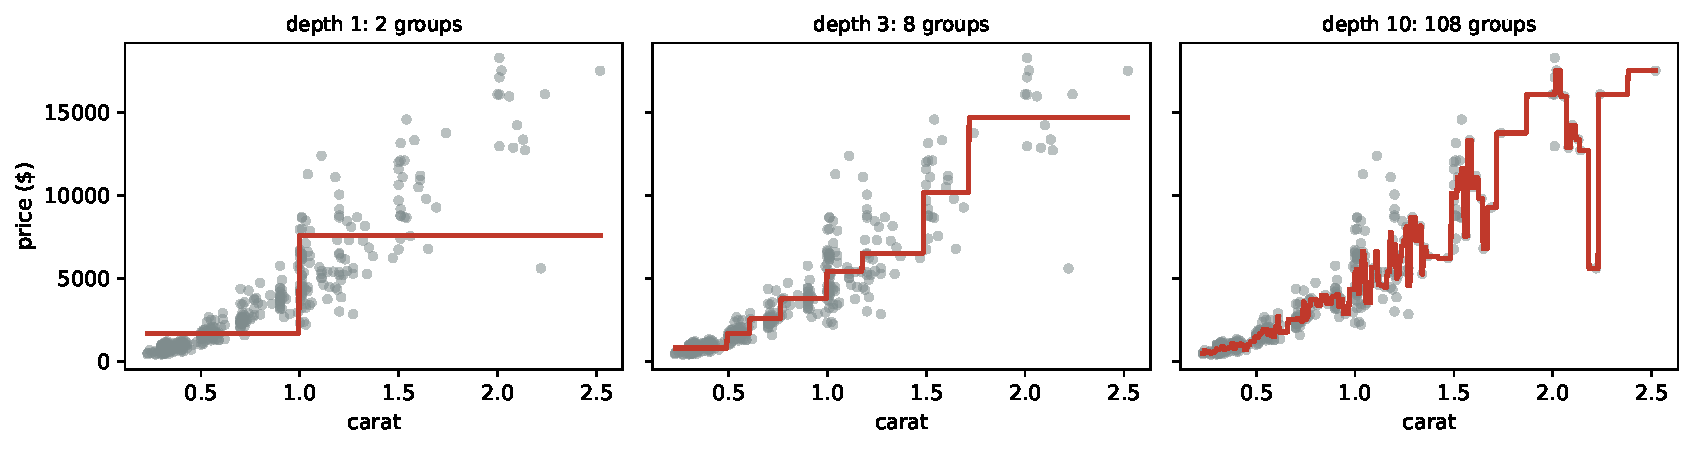
\includegraphics[width=\textwidth]{fig_u5_tree_steps.pdf}
\vspace{0.3em}
\begin{minipage}{0.94\textwidth}\small
One split gives two steps. Three levels give eight groups and a recognisable staircase. Ten
levels give a step for almost every handful of jobs, which is the tree memorising this sample.
\end{minipage}
\end{frame}

\begin{frame}{Reading a fitted tree}
\centering
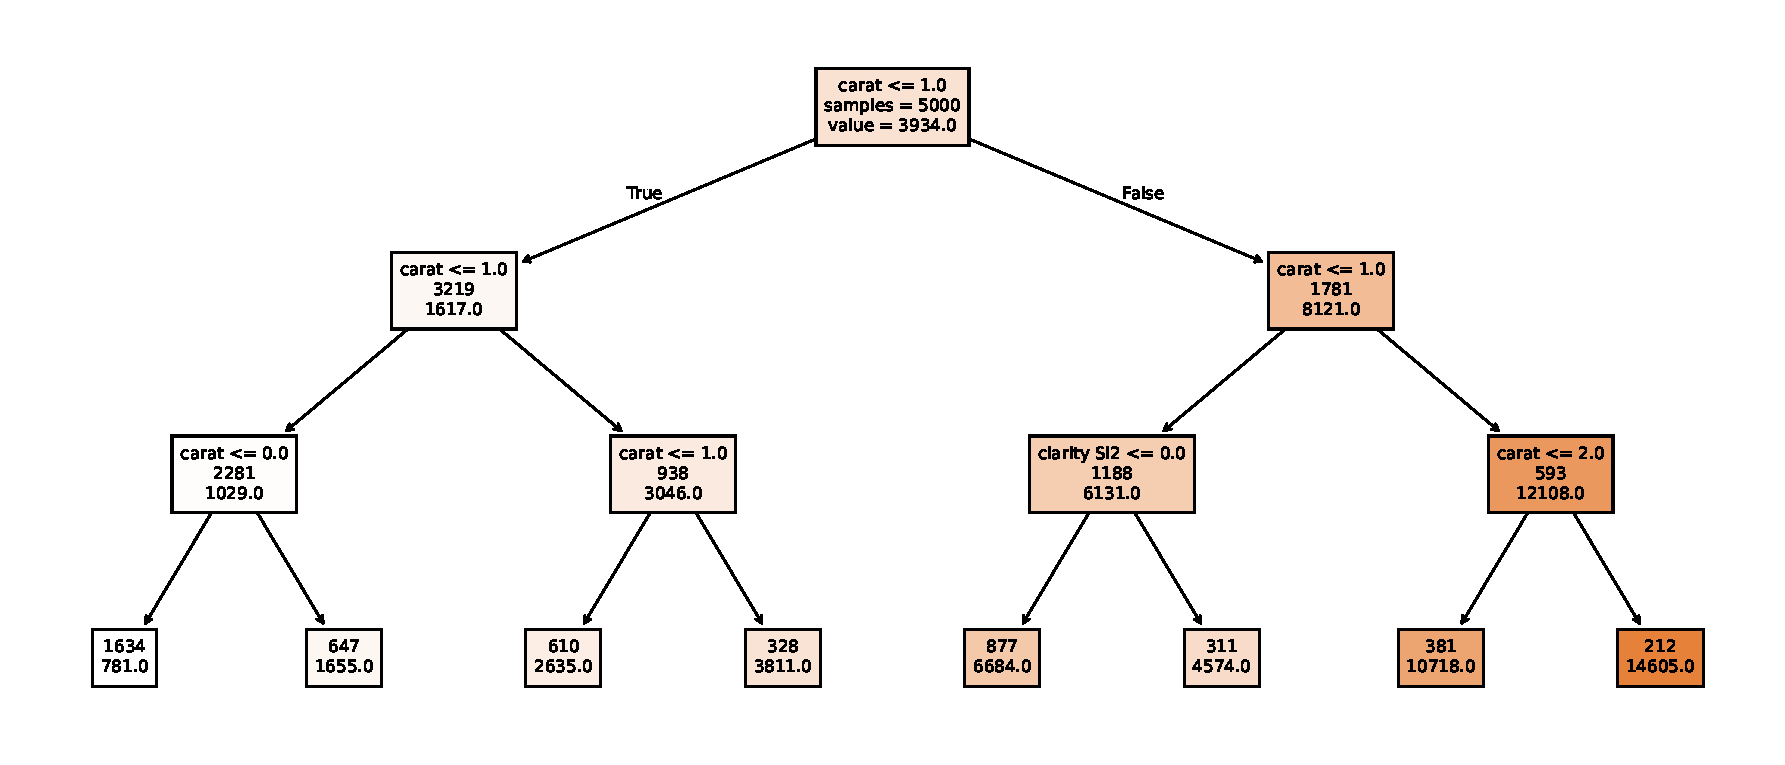
\includegraphics[width=0.92\textwidth]{fig_u5_tree_diagram.pdf}
\end{frame}

\begin{frame}{The same tree, out loud}
\begin{itemize}
  \item The first question is lot size, at about 11,000 square feet. Size matters more than
        anything else here, which matches the regression.
  \item Inside the small-lot branch, the next question is \textbf{the gate}. Gated properties take
        noticeably longer at the same size.
  \item Inside the large-lot branch, the tree asks about \textbf{crew size} and then about
        \textbf{steep slope}. Slope appears only on large lots.
  \item Each box at the bottom holds a group of jobs and predicts their average.
\end{itemize}
\begin{principle}{what a tree is}
A set of rules that partition the data, and one number per region. No coefficients, no equation,
and nothing that can be read as the effect of a variable.
\end{principle}
\end{frame}

\begin{frame}{How deep to go}
\begin{columns}[c]
\begin{column}{0.58\textwidth}
\centering
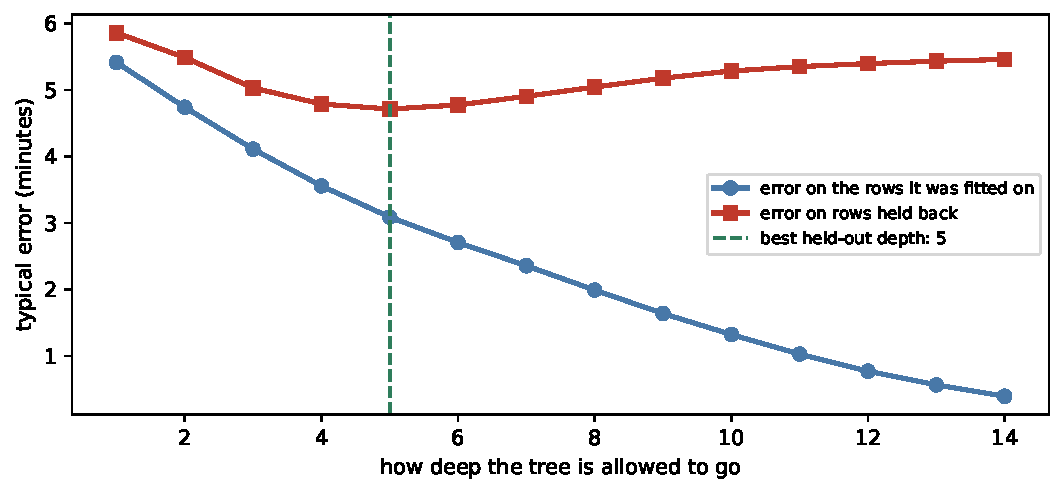
\includegraphics[width=\textwidth]{fig_u5_tree_depth.pdf}
\end{column}
\begin{column}{0.42\textwidth}
\small
\begin{itemize}
  \item Error on the fitted rows falls with every level and keeps falling. A deep enough tree
        fits them exactly.
  \item Held-out error bottoms out around depth 5 and then climbs.
  \item Depth is this model's complexity dial, and it is chosen the same way as everything in
        Unit 4: on data the tree did not see.
\end{itemize}
\end{column}
\end{columns}
\end{frame}

\begin{frame}{What trees are good at, and bad at}
\begin{center}\small
\begin{tabular}{L{0.44\textwidth} L{0.44\textwidth}}
\toprule
\textbf{Good at} & \textbf{Bad at} \\
\midrule
thresholds, where something changes at a value & smooth trends, which it approximates with stairs \\
interactions, free of charge, because every split happens inside an earlier split & giving you an
effect size with an interval \\
predictors on any scale, with no transformation needed & stability: a few different rows can
change the top split \\
mixed types of predictor in one model & anything outside the range of the data \\
\bottomrule
\end{tabular}
\end{center}
\end{frame}

\begin{frame}{The extrapolation problem, in one line}
\begin{itemize}
  \item A tree predicts the average of the training jobs in a region. For a lot bigger than any
        it has seen, it returns the average of the biggest group it knows.
  \item A line at least continues in a direction. A tree flattens out completely.
  \item Neither is trustworthy out there, but they fail differently, and the tree fails silently.
\end{itemize}
\end{frame}

\begin{frame}{Forests and boosting, in one slide}
\begin{itemize}
  \item A single tree is unstable. \textbf{Random forests} fit many trees to resampled data and
        average them. \textbf{Boosting} fits trees in sequence, each correcting the last.
  \item Both usually predict better than one tree, and both give up the one thing a single tree
        had: you could read it.
  \item We are not going further than naming them. Unit 2 put them on the menu, and this is where
        they come from.
\end{itemize}
\end{frame}

\begin{frame}{Your turn \#2}
\begin{yourturn}{what would the tree do?}
A tree is fitted to predict mowing time. Its first split is \emph{lot size above 11,000 sq ft},
and inside the small-lot branch it splits on \emph{gated}.
\vspace{0.3em}

A new job comes in: a 2,000 square foot lot, behind a gate. What does the tree predict, roughly,
and what would a regression with a gate coefficient predict differently?
\end{yourturn}
\end{frame}

\begin{frame}{Your turn \#2: answer}
\begin{itemize}
  \item The tree sends the job left at the first question, then right at the gate question, and
        predicts the average of the small gated jobs it has seen.
  \item A regression adds a gate coefficient to whatever the size term gives, so the gate costs
        the same percentage on a tiny lot as on a large one.
  \item Which is right depends on the gate: if it is a fixed walk from the street, the tree's
        version is closer. That is a question about mowing, not about statistics.
\end{itemize}
\end{frame}

% ======================================================================
\section{Trees as a scout}
% ======================================================================
\begin{frame}{Using a tree to improve a regression}
\begin{itemize}
  \item A tree will not give you an effect with an interval, so it cannot be the thing you
        report when the question is how much something matters.
  \item But it searches shapes you would never check by hand, and its splits are hypotheses
        written in a readable form.
  \item So: fit the tree, read the structure, and put what it found into the regression.
\end{itemize}
\begin{principle}{scout and report}
Let the tree tell you where to look. Let the regression tell you how much, and how sure.
\end{principle}
\end{frame}

\begin{frame}{What this tree was telling us}
\begin{itemize}
  \item \textbf{A split on gated, inside one size branch.} The gate costs time, and it is worth a
        term of its own.
  \item \textbf{A split on steep slope only inside the large-lot branch.} Slope seems to matter
        on big lots and not on small ones. In regression language, that is an interaction between
        size and slope.
  \item \textbf{Splits on lot size at several places.} The relationship with size is not a
        straight line, which the log already told us.
\end{itemize}
\end{frame}

\begin{frame}{The hint, checked}
\begin{columns}[c]
\begin{column}{0.56\textwidth}
\centering
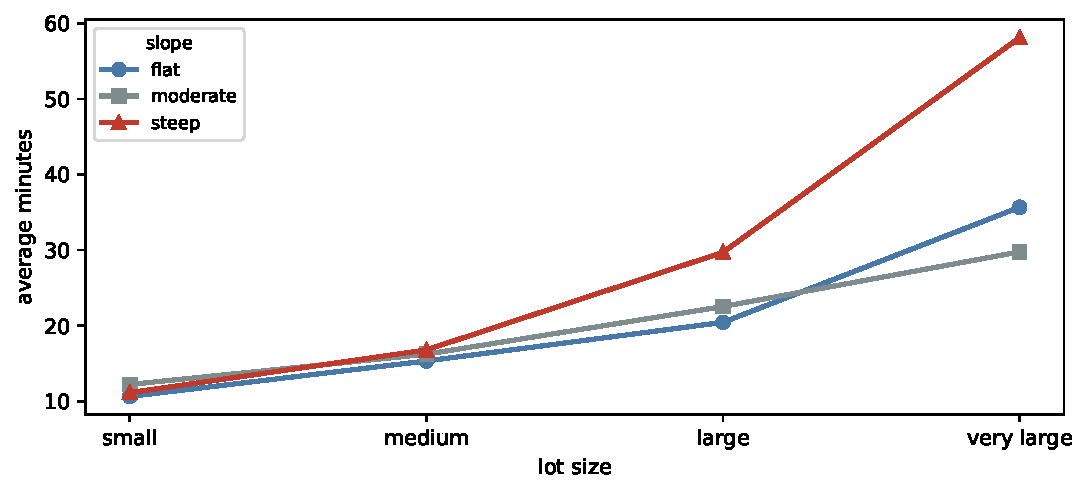
\includegraphics[width=\textwidth]{fig_u5_interaction.pdf}
\end{column}
\begin{column}{0.44\textwidth}
\small
Average minutes by lot size band and slope.
\begin{itemize}
  \item On small and medium lots the three slopes cost about the same.
  \item On large and very large lots, steep pulls away from the others.
  \item That is what the tree saw when it split on slope only inside the large branch.
\end{itemize}
\end{column}
\end{columns}
\end{frame}

\begin{frame}{Put it in the model}
Add one interaction, between $\log(\text{lot size})$ and steep, to the log model:
\begin{center}\small
\begin{tabular}{lccc}
\toprule
\textbf{Model} & \textbf{$R^2$} & \textbf{AIC} & \textbf{cross-validated error} \\
\midrule
line on raw size & & & 0.236 \\
log size, log minutes & 0.742 & $-215$ & 0.208 \\
\quad plus size $\times$ steep & \textbf{0.745} & $\mathbf{-223}$ & \textbf{0.207} \\
\midrule
the tree on its own (depth 5) & & & 0.253 \\
\bottomrule
\end{tabular}
\end{center}
\begin{itemize}\small
  \item The interaction the tree pointed at is real: $p = 0.0016$, and AIC improves by 8.
  \item The regression that took the hint predicts better than the tree that gave it.
\end{itemize}
\end{frame}

\begin{frame}{Why end here}
\begin{itemize}
  \item The tree is a fast, honest search for structure you did not think to look for.
  \item The regression turns what it finds into a number with an interval, in units somebody can
        act on.
  \item Used together they cover each other's weakness, and you can defend every term in the
        final model by saying where it came from.
\end{itemize}
\begin{trap}{the step you cannot skip}
A term suggested by a tree was still suggested by looking at the data. Check it on held-out rows,
and say in the write-up that this is where it came from.
\end{trap}
\end{frame}

% ======================================================================
\section{LLM check}
% ======================================================================
\begin{frame}{LLM check: mistake or not? (1 of 2)}
\begin{llmcheck}{we asked about a fan in the residuals}
\textbf{We told it:} ``My residuals fan out as the fitted values grow. What should I do?''\\[4pt]
\textbf{It answered:} ``Remove the outliers at the high end and refit. That will stabilise the
variance and improve your $R^2$.''
\end{llmcheck}
\vspace{0.2em}
\centering\small Mistake, or no mistake? Decide before we click.
\onslide<2->{%
\begin{trap}{verdict: mistake}
A fan is not an outlier problem. The large cases are not errors, they are simply more variable,
and deleting them changes the question the model answers. Model the log instead.
\end{trap}}
\end{frame}

\begin{frame}{LLM check: mistake or not? (2 of 2)}
\begin{llmcheck}{we asked it to read a tree}
\textbf{We told it:} ``My tree splits on gated right after lot size. What does that tell me?''\\[4pt]
\textbf{It answered:} ``Gating is the second most important driver of mowing time. The split
suggests it matters within a size range, so it may be worth testing a gate term, or a gate by
size interaction, in a regression where you can put a number on it.''
\end{llmcheck}
\vspace{0.2em}
\centering\small Mistake, or no mistake?
\onslide<2->{%
\begin{principle}{verdict: no mistake}
The second sentence is exactly the move this unit ends on. The phrase ``second most important''
is loose, but it stops short of calling the split an effect.
\end{principle}}
\end{frame}

% ======================================================================
\section{Consolidate}
% ======================================================================
\begin{frame}{What to do when a line is not enough}
\small
\begin{enumerate}
  \item \textbf{Plot the residuals} against the fitted values, every time.
  \item \textbf{Name what you see:} cloud, curve, fan, or one point.
  \item \textbf{Curve:} add a squared term, or transform the predictor.
  \item \textbf{Fan:} model the log of the outcome, and report in percentages.
  \item \textbf{One point:} find out what it is before touching it.
  \item \textbf{Not independent, or not a number:} name the right family and get help.
  \item \textbf{Out of ideas:} fit a shallow tree and read its splits for terms to try.
  \item \textbf{Check any term you found this way} on data the search did not touch.
\end{enumerate}
\end{frame}

\begin{frame}{The traps, all in one place}
\begin{trap}{the ones that bite most often}
\begin{itemize}
  \item Reading coefficients from a model whose residuals are patterned.
  \item Reporting a coefficient from a logged model in the original units.
  \item Using $\log(y+1)$ on zeros because it ran without complaining.
  \item Deleting an inconvenient point and not saying so.
  \item Calling a tree's split an effect, or its variable ranking an effect size.
  \item Asking a tree to predict outside the range of its training data.
  \item Comparing a tree and a regression on the rows both were fitted on.
  \item Adding a tree-suggested term and reporting its p-value as if you had planned it.
\end{itemize}
\end{trap}
\end{frame}

\begin{frame}{What you should be able to do with software}
\small
\begin{center}\footnotesize
\begin{tabular}{p{0.44\textwidth} p{0.46\textwidth}}
\toprule
\textbf{You should be able to} & \textbf{What you would reach for} \\
\midrule
Plot residuals against fitted values & \texttt{plt.scatter(fit.fittedvalues, fit.resid)} \\
Model a logged outcome & \texttt{smf.ols("np.log(y) $\sim$ x", data)} \\
Add a curve & \texttt{smf.ols("y $\sim$ x + I(x**2)", data)} \\
Add an interaction & \texttt{smf.ols("y $\sim$ x * group", data)} \\
Fit a shallow tree & \texttt{DecisionTreeRegressor(} \newline
\texttt{\phantom{xx}max\_depth=3).fit(X, y)} \\
Read the tree & \texttt{export\_text(tree, feature\_names=...)} \\
Choose the depth & \texttt{cross\_val\_score} over a few depths \\
\bottomrule
\end{tabular}
\end{center}
\end{frame}

\begin{frame}{Where we go next}
\begin{itemize}
  \item That closes the modelling half of the course. You can fit a model, read it, check it,
        repair it, choose between candidates, and predict with honest error bars.
  \item \textbf{Unit 6} starts the machinery underneath all of it: probability, and what chance
        alone produces.
  \item Everything from here gives a reason for the tools you have been using, and then puts them
        to work on outcomes that are not continuous numbers.
\end{itemize}
\end{frame}

\end{document}
